\documentclass{article}
\usepackage{amsmath}
\usepackage{tikz}
\usetikzlibrary{shapes.geometric, arrows.meta, positioning}

\begin{document}

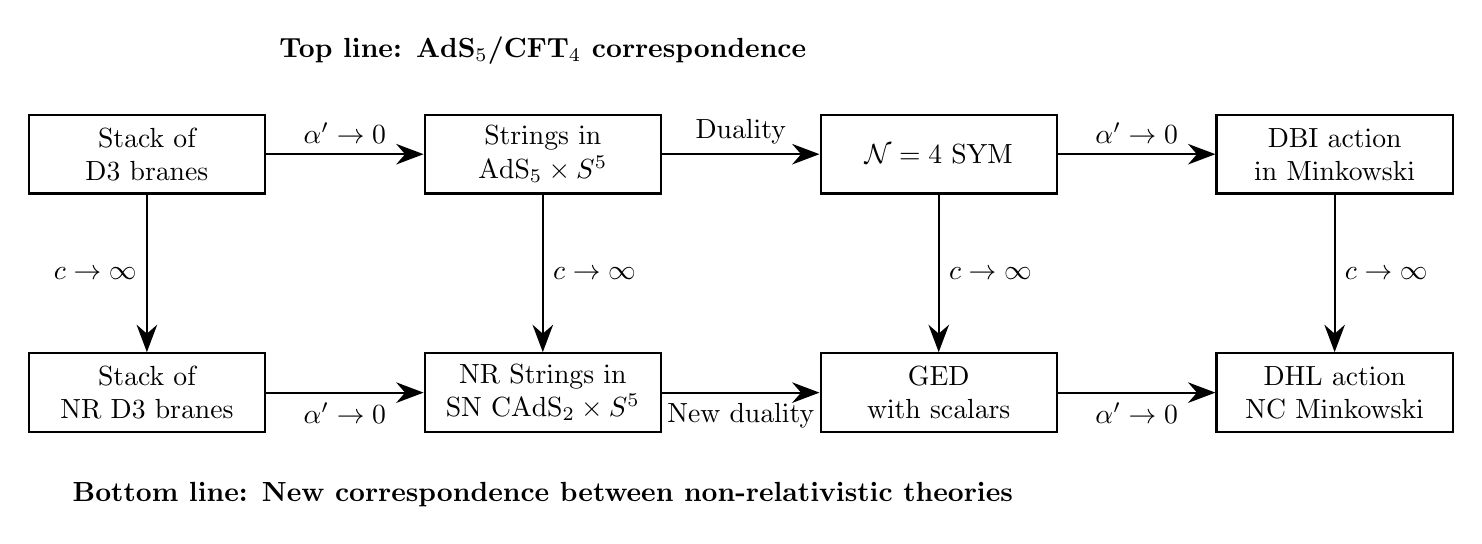
\begin{tikzpicture}[
    node distance=2cm,
    block/.style={rectangle, draw, thick, minimum width=3cm, minimum height=1cm, align=center},
    arrow/.style={-{Stealth[scale=1.5]}}
]

% Top row nodes
\node[block] (d3branes) {Stack of\\ D3 branes};
\node[block, right=of d3branes] (strings_ad5_s5) {Strings in\\ ${\rm AdS}_5\times S^5$};
\node[block, right=of strings_ad5_s5] (n4sym) {$\mathcal{N}=4$ SYM};
\node[block, right=of n4sym] (dbi_min) {DBI action\\ in Minkowski};

% Bottom row nodes
\node[block, below=of d3branes] (nr_d3branes) {Stack of\\ NR D3 branes};
\node[block, below=of strings_ad5_s5] (nr_strings) {NR Strings in\\ SN CAdS${}_2\times S^5$};
\node[block, below=of n4sym] (ged_scalars) {GED\\ with scalars};
\node[block, below=of dbi_min] (nc_dbi) {DHL action\\ NC Minkowski};

% Arrows for top row
\draw[arrow, thick] (d3branes) -- node[above] {$\alpha^\prime\to 0$} (strings_ad5_s5);
\draw[arrow, thick] (strings_ad5_s5) -- node[above] {Duality} (n4sym);
\draw[arrow, thick] (n4sym) -- node[above] {$\alpha^\prime\to 0$} (dbi_min);

% Arrows for bottom row
\draw[arrow, thick] (nr_d3branes) -- node[below] {$\alpha^\prime\to 0$} (nr_strings);
\draw[arrow, thick] (nr_strings) -- node[below] {New duality} (ged_scalars);
\draw[arrow, thick] (ged_scalars) -- node[below] {$\alpha^\prime\to 0$} (nc_dbi);

% Vertical arrows connecting top and bottom rows
\draw[arrow, thick] (d3branes.south) -- node[left] {$c\to\infty$} (nr_d3branes.north);
\draw[arrow, thick] (strings_ad5_s5.south) -- node[right] {$c\to\infty$} (nr_strings.north);
\draw[arrow, thick] (n4sym.south) -- node[right] {$c\to\infty$} (ged_scalars.north);
\draw[arrow, thick] (dbi_min.south) -- node[right] {$c\to\infty$} (nc_dbi.north);

% Additional labeling (optional)
\node[above=0.5cm of strings_ad5_s5] {\textbf{Top line: AdS${}_5$/CFT${}_4$ correspondence}};
\node[below=0.5cm of nr_strings] {\textbf{Bottom line: New correspondence between non-relativistic theories}};

\end{tikzpicture}

\end{document}